\documentclass{article}
% Change "article" to "report" to get rid of page number on title page
\usepackage{amsmath,amsfonts,amsthm,amssymb}
\usepackage{setspace}
\usepackage{Tabbing}
\usepackage{fancyhdr}
\usepackage{lastpage}
\usepackage{extramarks}
\usepackage{chngpage}
\usepackage{soul,color}
\usepackage{graphicx,float,wrapfig}
\usepackage{xcolor}
\usepackage{textcomp}
\usepackage{listings}
\usepackage[section]{placeins}
\usepackage{afterpage}


\usepackage{caption}
\DeclareCaptionFont{white}{\color{white}}
\DeclareCaptionFormat{listing}{\colorbox{gray}{\parbox{\textwidth}{#1#2#3}}}
\captionsetup[lstlisting]{format=listing,labelfont=white,textfont=white}

% In case you need to adjust margins:
\topmargin=-0.45in      %
\evensidemargin=0in     %
\oddsidemargin=0in      %
\textwidth=6.5in        %
\textheight=9.0in       %
\headsep=0.25in         %

\setlength{\parindent}{1cm}


\lstset{language=C,tabsize=3,frame=lines,keywordstyle=\color{blue},commentstyle=\color{purple},stringstyle=\color{red},numbers=left,numberstyle=\tiny,numbersep=5pt,breaklines=true,showstringspaces=false,basicstyle=\footnotesize,emph={label}}


% Document Specific Information
\newcommand{\Title}{Succincter}
\newcommand{\Date}{Tuesday,\ December\ 11,\ 2012}
\newcommand{\Class}{Computer Science 222}
\newcommand{\ClassTime}{}
\newcommand{\ClassInstructor}{Professor Mitzenmacher}
\newcommand{\AuthorName}{Dan Bradley (dbradley@college), Saagar Deshpande (sdeshpande@college)}

% Setup the header and footer
\pagestyle{fancy}                                                       %
\lhead{Bradley, Deshpande}                                                 %
%\chead{\Class\ (\ClassInstructor\ \ClassTime): \Title}  %
\chead{\Title}  %
\rhead{\Date}                                                     %
\lfoot{\lastxmark \Class}                                                      %
\cfoot{}                                                                %
\rfoot{Page\ \thepage\ of\ \pageref{LastPage}}                          %
\renewcommand\headrulewidth{0.4pt}                                      %
\renewcommand\footrulewidth{0.4pt}                                      %

% This is used to trace down (pin point) problems
% in latexing a document:
%\tracingall


%%%%%%%%%%%%%%%%%%%%%%%%%%%%%%%%%%%%%%%%%%%%%%%%%%%%%%%%%%%%%
% Make title
\title{\textmd{\textbf{\Class:\ \Title}}\\\normalsize\vspace{0.1in}\small{ \Date}\\\vspace{0.1in}\large{\textit{\ClassInstructor\ \ClassTime}}}
\author{\textbf{\AuthorName}}
\date{Final Project}
%%%%%%%%%%%%%%%%%%%%%%%%%%%%%%%%%%%%%%%%%%%%%%%%%%%%%%%%%%%%%

\begin{document}

\maketitle

\bigskip
\centerline{**********}

\noindent \section{Abstract}
Using Mihai Patrascu's 2008 paper "Succincter" [1],  we implement a way to store trits (trinary values) within 1.01\% of the ideal space of $n*log_2(3)$ while having lookup in $O(t)$ time, where $t$ is the depth of our data structure. We find that this is both a fast and space efficient data structure with room for extension past simply storing trits.

\noindent \section{Introduction}

\indent There are few effective methods for storing trits. In this paper, we focus on three of them: the naive method, arithmetic coding, and our succincter implementation.\\
\indent The naive method is simple. As a trit has more information than a bit, but less than two bits, store each trit using two bits. Obviously this is not the most space-efficient method, you could encode $\frac{4}{3}$ as much information in the same space, so it is clearly wasteful. It is however, very fast, both on encode and decode. Encode is strictly linear, with very small constants. The encoder we used took 3.9 milliseconds to encode 500000 entries, and 13.7 milliseconds to decode 500000 entries.\\
\indent Arithmetic coding is much more effective at reducing size. By reducing the entries to one number, we can encode in exactly $\lceil \frac{n*log_2(3)}{8}\rceil$ bytes. Decoding, however, ideally takes linear time, as to reach any original entry, you must go through every entry prior, there is no way to randomly access any element. Furthermore, the nature of arithmetic coding lends itself to manipulation of large numbers, which is time consuming.\\
\indent The succincter data structure is a recursive approach to the problem, and attempts to approach the ideal space usage without sacrificing on decoding time, especially for individual entries. Essentially, succinter takes an array of entries, and breaks them into blocks. These blocks are each treated as one large number, base $K$ (in the first level of the structure when storing trits $K$ is 3, but $K$ changes by level). These large number are then divided by $2^M$ where $M$ is a user-defined variable. The remainder is stored for transmission, and the quotient gets passed up to the next level of the data structure as a new array. The quotient will be some number $\{0 , 1, 2, ... , K -1\}$, and so we can repeat the process on the new array by simply finding new blocks and treating them as numbers base $K$.\\
\indent Mihai Patrascu outlined the idea of succinter data structures in [1], but we took some liberties with our implementation, as his approaches to finding block size and $K$ proved less useful in practice than they might have been in theory.

\noindent \section{Implementation}
\emph{ENCODING}\\
To encode, we start with an array with fixed size of trits with pseudorandomly assigned values. For the sake of simplicity, and the fact that the values of the trits do not particularly matter for our inquiry, we used the $c$ standard library rand() function seeded by the time of running. \\

We also decided that all remainders would be up to 32 bits long, which for the sake of discussion we will refer to as $M$.\\

With the size of the array and the base 3, we construct the necessary headers to be used by the decoder, specifically the size of the array at that level, the base at that level, and the block size at that level. \\

Given the size and base, the header of all levels are constructable. We are trying to fill an array of size LEVELS (an arbitrary constant we the user decide) + 1 with the size for that level, the block size fro that level, and the base for that level. In the context of this paper, we will call this array headers. We find an $n$ such that our new $K = \lceil \frac{3^n}{2^M} \rceil > 2$. $n$ is the block size for the level, the base for the level is the old $K$, and the size for the level is the old size. The variables then update, with old $K$ being set to new $K$, size decreasing by a factor chunksize, and we are back where we started, just a level higher up the headers.\\

Once the headers are found, we can begin to encode the actual data. We encode recursively, starting from the bottom level = 0 and continuing until level equals LEVELS. To encode, we are given an array to encode, we take the first headers[level].chunksize entries, and combine them into one large number. We then divide by $2^M$, store the remainder, and pass the quotient to a new array we're building for the next level. We do this for each block, and when we reach the end of our entries, we call decode again, on the new array, with level increased.\\

Eventually level will equal LEVELS, and when it does, we naively code the array: we figure out how many bits it takes to completely store a number base $K$, and store each number in the array using that many bits. \\

We put in an output file the SIZE, LEVELS, and M, write all the headers to the file, then write out all the bits for the last level of storage. \\\\

\noindent\emph{DECODING}\\
For both decoding schemes, we first need to read and interpret the input file, which is done essentially in reverse of encoding, taking SIZE, LEVELS, and M to be global variables, as well as the headers array, an array of all the remainders, and the last array that was encoded.

\indent \textbf{Decode All}
We are given an array (to start with, the last arrray), and that we are on the highest level, and with that and the global variables, we can decode every original entry in the right order. To do this, we take the remainder corresponding to the index in the array the level below. 

\indent \textbf{Decode One}

\bigskip

\noindent \section{Results and Analysis}

We ran our implementation of Succincter on 500000 trits except in the case of individual decoding, where we only use 200000 trits. We compared this implementation against a simple C implementation of arithmetic encoding as well as a naive C implementation of a trit to bit converter, which stores each trit as its corresponding bit.

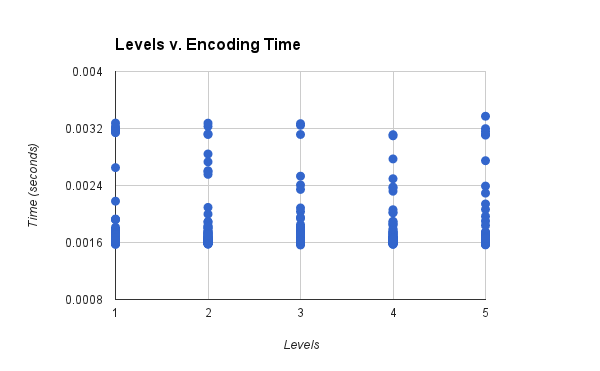
\includegraphics[scale=0.4]{images/betterlevel_v_encode}
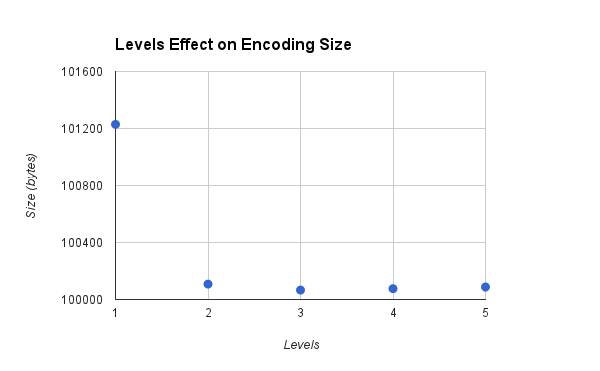
\includegraphics[scale=0.4]{images/lvl_encodingsize}
\afterpage{\vfill}

Initially, we compared the speed of encoding and decoding at each level as well as the space required for the encoding process. We noticed that the encoding time is relatively similar for each of the levels we run Succincter on, with level 4 edging the others by an insignificant amount. This indicates that the time taken is relatively the same for any level of encoding. The reason that we see the high levels of encoding to be slightly faster is because the last layer of values need to be specially encoded from their current base to bits. For the lower levels, this is a more expensive process as the number of values left to be specially encoded in larger. However, this time is still largely insignificant for large sets of values. \\

This reasoning for the encoding time also extends to the average encoding sizes we see in our experimentation. We see that as the level increases, we have an immediate decrease in size from level 1 to level 2, and after that the size remains roughly the same. This indicates that the size of the encoded data will remain the same for any level past level 1, which makes the data structure extremely scalable in both time and space. 

\begin{center}\smallskip
    \begin{tabular}{ | c | c | c | c |}
    \hline
    Level & Avg. Encode Time (sec) & Avg. Decode Time (sec) & Avg. Encode Size (bytes) \\ \hline
    1 & 0.00178906 & 0.043107825396825 & 101229\\
    2 & 0.00177046 & 0.041240047619048 & 100108\\
    3 & 0.00173798 & 0.041672920634921 & 100066\\
    4 & 0.00173344 & 0.041674126984127 & 100076\\
    5 & 0.00175082 & 0.040755396825397 & 100088\\ \hline
    \end{tabular}
\end{center}



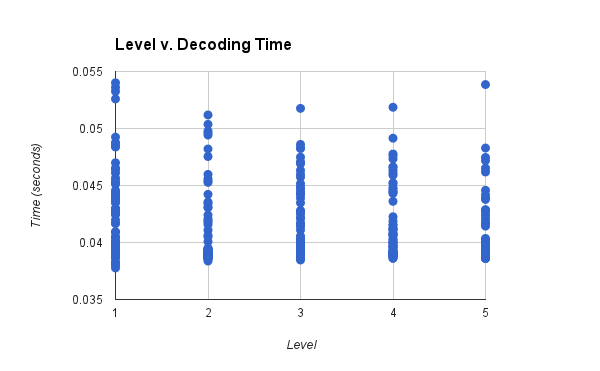
\includegraphics[scale=0.4]{images/betterlevel_v_decode}
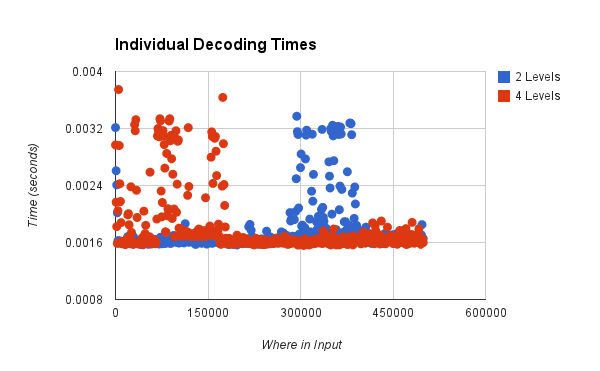
\includegraphics[scale=0.4]{images/individual_decodetime}
\afterpage{\vfill}

asdfaksdjf;aksldfjadsf\\
asdfaksdjf;aksldfjadsf\\
asdfaksdjf;aksldfjadsf\\


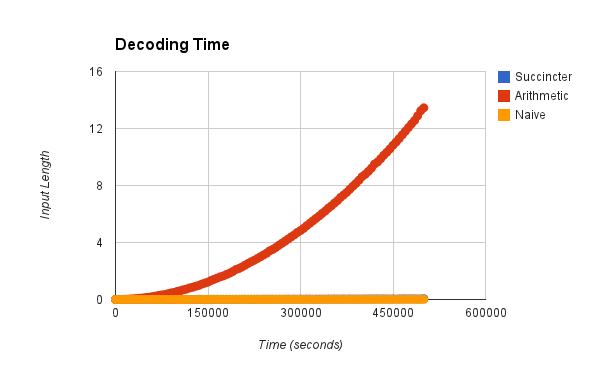
\includegraphics[scale=0.4]{images/decoding_time}
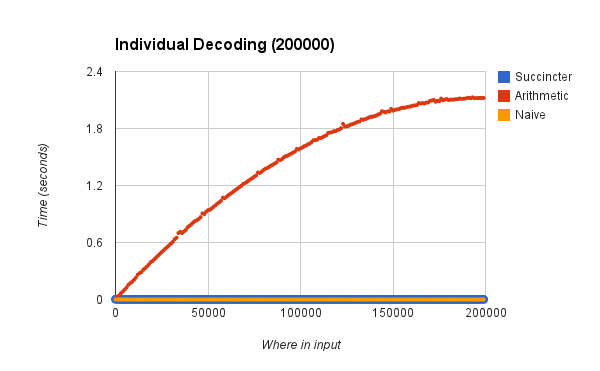
\includegraphics[scale=0.4]{images/individual_decode_20000}
\afterpage{\vfill}

asdfaksdjf;aksldfjadsf\\
asdfaksdjf;aksldfjadsf\\
asdfaksdjf;aksldfjadsf\\
asdfaksdjf;aksldfjadsf\\

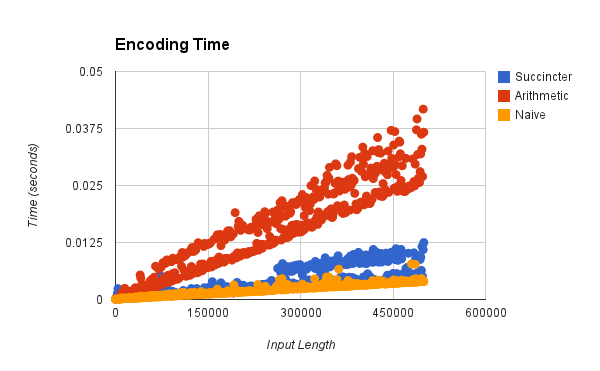
\includegraphics[scale=0.4]{images/encoding_time}
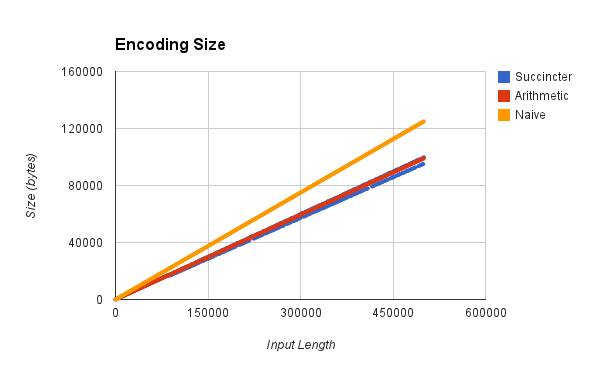
\includegraphics[scale=0.4]{images/encoding_size}
\afterpage{\vfill}

asdfaksdjf;aksldfjadsf\\


\noindent \section{Conclusion}

\bigskip
\centerline{**********}

\noindent \section{References}


\noindent \section*{Appendix}

%\lstinputlisting[language=C,label=problem4,caption=Code for Problem 4]{../succinct_code/encoder.c}

%\lstinputlisting[language=java,label=problem5,caption=Code for Problem 5]{countmin.java}

%\begin{lstlisting}[language=java,label=some-code,caption=Some Code]
% Connection db = DriverManager.getConnection("jdbc:h2:rel.db", "user", "pass");
%  Statement stmt = db.createStatement();
%  stmt.execupdate("INSERT INTO CAMPAIGN VALUES ('C1R1R2R3R4R5R6', 1234, 1170, 1189, 1934)");
%\end{lstlisting}
\end{document}

%%%%%%%%%%%%%%%%%%%%%%%%%%%%%%%%%%%%%%%%%%%%%%%%%%%%%%%%%%%%%

